%\documentclass[graybox,envcountchap,sectrefs]{svmono}
\ifx\nameofpaper\undefined
  \usepackage{macro_natsuume}
  \def\beginsection{\section*}
  \def\endofsection{\end{document}}
  \input draft_header.tex
\else
  \def\beginsection{\chapter}
  \def\endofsection{\endinput}
\fi

%\newcommand{\prerequisite}[1]{{\color{red} Advanced section prerequisite: #1}}
%\newcommand{\prerequisite}[1]{\textcolor{red}{Advanced section prerequisite: #1}}
\newcommand{\prerequisite}[1]{\textit{Advanced section prerequisite: #1}}
\newcommand{\ketc}{\ket_c}


%%%%%%%%%
\chapter{Exercises}\label{chap:exercise}
%\chapter*{Exercises}\label{chap:exercise}
%%%%%%%%%
%\addcontentsline{toc}{chapter}{Exercises}
\begin{prob}
%\label{prob:}
%\textbf{}\\
Find errors in this textbook as many as possible, and report to the author.
\end{prob}

%%%%%%%%%
\section*{Chap.~3}%\label{sec:}
%%%%%%%%%
%\setcounter{chapter}{3}
%\setcounter{prob}{0}

% Use the following environment.
% Don't forget to label each problem;
% the label is needed for the solutions' environment

\begin{prob}
%\label{prob1}
\textbf{Thermodynamic quantities of higher-dimensional Schwarzschild black holes}\\
Verify Eqs.~\eqref{eq:temp_Sch_d} and \eqref{eq:entropy_Sch_d}.
\end{prob}

\begin{prob}
%\label{prob1}
\textbf{Thermodynamic quantities of the RN black holes}\\
Verify Eqs.~\eqref{eq:temp_RN} and \eqref{eq:entropy_RN}.
\end{prob}

%%%%%%%%%
\section*{Chap.~5}%\label{sec:}
%%%%%%%%%
%\setcounter{chapter}{3}
%\setcounter{prob}{0}

\begin{prob}
%\label{prob1}
\textbf{Maxwell theory in $d$-dimensions} \\
\prerequisite{\sect{weyl_inv} } \\
Compute the energy-momentum tensor and its trace for
\be
%
\action = - \frac{1}{4e^2} \int d^dx\, F^{\mu\nu}F_{\mu\nu}~.
%\label{eq:}
%
\ee
The trace does not vanish except $d=4$. But the trace vanishes up to a total derivative:
\be
%
T^{\mu}_{~\mu} = \frac{4-d}{4e^2} F^2 = \frac{4-d}{2e^2} \del_\mu(A_\nu F^{\mu\nu})~,
%\label{eq:}
%
\ee
where we use the equation of motion in the last equality. Then, the Maxwell theory is scale invariant according to \sect{weyl_inv}. Comparing with \eq{virial}, $K^\mu = (4-d) A_\nu F^{\mu\nu}/(2e^2)$.

However, $K^\mu$ is not a divergence, so the Maxwell theory is scale invariant but is not conformal invariant when $d\neq4$.

\end{prob}

\begin{prob}
%\label{prob1}
\textbf{Local Weyl invariant scalar theory in $d$-dimensions} \\
\prerequisite{\sect{weyl_inv} } \\
Show that $T_{\mu\nu}$ \eqref{eq:EM_scalar_conf} is traceless when $\xi=(d-2)/4(d-1)$.
\end{prob}


%%%%%%%%%
\section*{Chap.~6}%\label{sec:}
%%%%%%%%%
%\setcounter{chapter}{3}
%\setcounter{prob}{0}

\begin{prob}
%\label{prob1}
\textbf{The $H^2$, AdS$_2$, and dS$_2$ metric}\\
Verify Eqs.~\eqref{eq:metric_h2}, \eqref{eq:metric_ads2}, and \eqref{eq:metric_ds2}.
\end{prob}

\begin{prob}
%\label{prob1}
\textbf{The AdS$_2$ metric in various coordinates}\\
Verify Eqs.~\eqref{eq:ads2_static}, \eqref{eq:ads2_conf}, and \eqref{eq:ads2_poincare}.
\end{prob}

\begin{prob}
%\label{prob:}
\textbf{\poincare\ patch}\\
Derive the region coved by \poincare\ coordinates, or the \poincare\ patch, in the AdS$_2$ spacetime  (\fig{AdS2_Penrose}). To do so, one has to know the relation between conformal coordinates $(\tg, \theta)$ and \poincare\ coordinates $(t,r)$. First, write $r$ in terms of embedding coordinates $(X,Y,Z)$, and rewrite the expression in terms of conformal coordinates.
\end{prob}

{\color{blue} 
\textit{Solution:}
\begin{align}
%
Z-Y &= r \\
&= \frac{1}{\cos\theta}(\cos\tau-\sin\theta)>0~,
%\label{eq:}
%
\end{align}
An inspection of this relation reproduces \fig{AdS2_Penrose}.
}

\begin{prob}
\label{prob:rindler}
\textbf{Flat spacetime in disguise 1: Rindler spacetime}\\
\noindent
(a) Consider the Minkowski spacetime:
\be
%
ds^2 = -dT^2+dX^2~.
%\label{eq:}
%
\ee
Show that the coordinate transformation
\be
%
\begin{split}
T &= \rho \sinh t~, \\
X &=\rho\cosh t
\end{split}
\label{eq:rindler_transf}
%
\ee
leads to 
\be
%
ds^2 = - \rho^2 dt^2 + d\rho^2~.
\label{eq:rindler2}
%
\ee
This is the Rindler spacetime. The $\rho=\text{(constant)}$ lines are hyperbolas, and the $t=\text{(constant)}$ lines are straight lines. They cover the region $X>|T|$ of the Minkowski spacetime (\fig{rindler}).

A further coordinate transformation $\rho=2r^{1/2}$ leads to \eq{rindler}:
\be
%
ds^2 = -r dt^2 + \frac{dr^2}{r}
%\label{eq:}
%
\ee
(up to a trivial scaling of $t \rightarrow t/2$).

\noindent
(b) Note that the Euclidean continuation of \eq{rindler2} takes the same form as the near-horizon metric \eqref{eq:polar}. Then, the near-horizon geometry of the Schwarzschild \bh should become the Rindler spacetime. Verify this explicitly. 

In the near-horizon limit, the coordinate transformation to the Kruskal coordinates \eqref{eq:kruskal} reduces to \eq{rindler_transf} with $T \propto v$ and $X \propto u$.

\noindent
(c) Suppose the constant $\rho=\rho_0$ line represents the world-line of an observer. One can check that his proper time $\tau$ is given by $\tau = \rho_0 t$. Compute the covariant acceleration $a^\mu = dx^\mu/d\tau$ and verify that $a^2 = \eta_{\mu\nu} a^\mu a^\nu$ is constant. Namely, the world-line represents a uniform accelerated observer with $a^2=1/\rho_0^2$.

\end{prob}

%%============
\begin{figure}[tb]
\centering
\subfigure[]{
\scalebox{0.55}{ 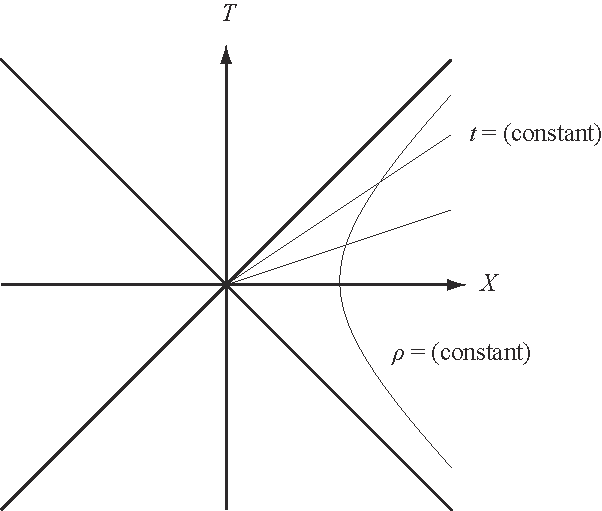
\includegraphics{Ch15_rindler.pdf} }
\label{fig:rindler}} \qquad
\subfigure[]{
\scalebox{0.55}{ 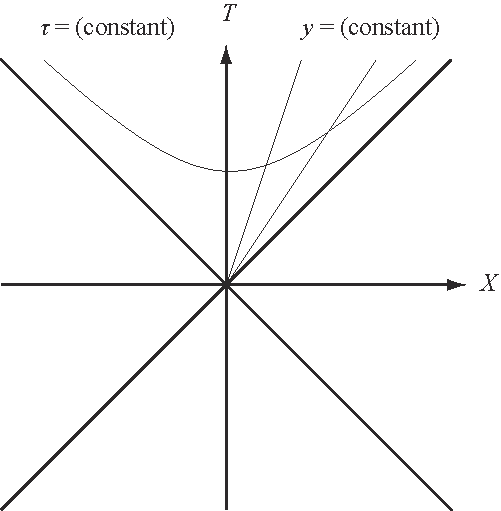
\includegraphics{Ch15_milne.pdf} }
\label{fig:milne}}
\vskip2mm
\caption{Flat spacetime in disguise.}
%\label{fig:path}
\end{figure}%
%%============

\begin{prob}
%\label{prob1}
\textbf{Flat spacetime in disguise 2: Milne universe}\\
Another flat spacetime in disguise is obtained by the coordinate transformation
\begin{align}
%
T &= \tau \cosh y~, \\
X &= \tau \sinh y~.
%\label{eq:}
%
\end{align}
Show that the metric in $(\tau, y)$ coordinates is given by
\be
%
ds^2 = - d\tau^2 + \tau^2 dy^2~.
\label{eq:milne}
%
\ee
This is known as the \keyword{Milne universe}. The metric \eqref{eq:milne} can be also obtained by the double Wick rotation from the Rindler spacetime \eqref{eq:rindler2}. 

The constant $y=y_0$ trajectory represents a boosted observer with Lorentz factor $ \gamma = \cosh y $ ($y := \tanh^{-1} v$ is known as \keyword{rapidity}.) 

The Milne universe may be regarded as a cosmological expansion. The constant $y=y_0$ trajectory represents the observer who experiences a universe expanding from the origin. 
%In general, a spatially flat cosmological solution is represented as
%\be
%
%ds^2 = -d\tau^2 + a(\tau)^2 d\bmx^2~,
%\label{eq:}
%
%\ee
%where $a(\tau)$ is known as the scale factor. In a cosmology, a fixed value of $\bmx$ represents, \eg, the position of each galaxy. 
%For the Friedmann-Robertson-Walker universe,  
%$a(\tau) \propto \tau^{2/3}$ (``dust-dominated universe"), 
%or $a(\tau) \propto \tau^{1/2}$ (``radiation-dominated universe"). 
%For the Milne universe, $a(\tau) \propto \tau$. 
The Milne universe is often used in the analysis of the QGP time evolution (\probset{bjorken}). In this sense, QGP can be regarded as a cosmological expansion.
\end{prob}


%%%%%%%%%
\section*{Chap.~7}%\label{sec:}
%%%%%%%%%
%\setcounter{chapter}{3}
%\setcounter{prob}{0}

\begin{prob}
%\label{prob1}
\textbf{Thermodynamic quantities of SAdS$_{p+2}$ black holes}\\
The SAdS$_{p+2}$ black hole is given by
\begin{align}
%
ds_{p+2}^2 &= - f dt^2  + \frac{dr^2}{f} + \left(\frac{r}{L}\right)^2 d\bmx_{p}^2~, \\
f &= \left(\frac{r}{L}\right)^2 \left\{ 1 - \left( \frac{r_0}{r} \right)^{p+1} \right\}~.
%\label{eq:}
%
\end{align}
Following \sect{sads_thermo}, compute the Hawking temperature of the black hole. Compute the other thermodynamic quantities using two methods below.\\
(a) (quick and dirty) 
Following \sect{sads_thermo}, compute $s$ from the area law, compute $\varepsilon$ from the first law, and compute $P$ and $F$ from the Euler relation.\\
(b) (\prerequisite{\sect{SAdS_free}})
Following \sect{SAdS_free}, compute $F$ from the on-shell action (bulk, Gibbons-Hawking, and counterterm actions).
\end{prob}

{\color{blue} 
\textit{Solution:}
\be
%
F = -\frac{V_p}{16\pi G_{p+2} L} \left( \frac{r_0}{L} \right)^{p+1}.
%\label{eq:}
%
\ee
}


%%%%%%%%%
\section*{Chap.~8}%\label{sec:}
%%%%%%%%%
%\setcounter{chapter}{3}
%\setcounter{prob}{0}

\begin{prob}
\label{prob:wilson_ads_soliton}
\textbf{Wilson loop in a confining phase}\\
\prerequisite{\sect{ads_soliton} } \\
Consider the AdS soliton geometry \eqref{eq:AdS_soliton}. Following \sect{wilson_details}, compute the quark potential, or the Wilson loop on the $t'$-$x$ plane, and verify \eq{wilson_ads_soliton}.
\end{prob}

{\color{blue} 
\textit{Solution:}
It is convenient to express results in dimensionless quantities. The quark separation $\calR$ is given by
\be
%
\frac{\calR}{l}
= \frac{2}{\pi}(1-\epsilon)^{1/4}
\int_1^\infty \frac{dy}{ \sqrt{(y^4-1)(y^4-1+\epsilon)} }~,
%\label{eq:}
%
\ee
%\be
%
%\frac{\calR}{2}
%= \frac{L^2}{\rmin}\sqrt{\epsilon}
%\int_1^\infty \frac{dy}{ \sqrt{(y^4-1)(y^4-1+\epsilon)} }~,
%\label{eq:}
%
%\ee
where $\epsilon:=1-(r_0/\rmin)^4$.
The potential energy is given by
\be
%
l \Delta E = \left(\frac{L}{l_s}\right)^2 \frac{1}{ (1-\epsilon)^{1/4} }
\left\{  
\int_1^\infty\left(\frac{y^4}{ \sqrt{(y^4-1)(y^4-1+\epsilon)} } -1 \right) dy - 1+ (1-\epsilon)^{1/4}
\right\}~,
%\label{eq:}
%
\ee
where $\Delta E :=E-E_0$. 

When $\epsilon \simeq 1$, $\calR \ll l$, \ie, the quark separation is shorter than the $S^1$ radius. In this case, one obtains the Coulomb potential. When $\epsilon \simeq 0$, $\calR \gg l$, and one obtains the confining potential. 
}

\begin{prob}
\label{prob:wilson_debye}
\textbf{Wilson loop at finite temperature} 
\cite{Rey:1998bq2,Brandhuber:1998bs2}\\
Consider the SAdS$_5$ geometry. Following \sect{wilson_details}, compute the quark potential, or the Wilson loop on the $t$-$x$ plane, and verify \eq{wilson_debye}.
\end{prob}

{\color{blue} 
\textit{Solution:}
The quark separation $\calR$ is given by
\be
%
T \calR
= \frac{2}{\pi}(1-\epsilon)^{1/4}\sqrt{\epsilon}
\int_1^\infty \frac{dy}{ \sqrt{(y^4-1)(y^4-1+\epsilon)} }~.
%\label{eq:}
%
\ee
%\be
%
%\frac{\calR}{2}
%= \frac{L^2}{\rmin}\sqrt{\epsilon}
%\int_1^\infty \frac{dy}{ \sqrt{(y^4-1)(y^4-1+\epsilon)} }~,
%\label{eq:}
%
%\ee
The potential energy is given by
\be
%
\frac{\Delta E}{T} = \left(\frac{L}{l_s}\right)^2 \frac{1}{ (1-\epsilon)^{1/4} }
\left\{  
\int_1^\infty \left(\sqrt{ \frac{y^4-1+\epsilon}{y^4-1} } -1 \right)dy - 1+ (1-\epsilon)^{1/4}
\right\}~.
\label{eq:potential_debye}
%
\ee
%\be
%
%E-E_0 = \frac{2}{2\pi l_s^2} \left\{ \rmin 
%\int_1^\infty \left(\sqrt{ \frac{y^4-1+\epsilon}{y^4-1} } -1 \right)dy - \rmin + r_0 
%\right\}~.
%\label{eq:}
%
%\ee

When $\epsilon \simeq 1$, $T\calR \ll 1$ (low temperature). In this case, one obtains the Coulomb potential. Now, decrease $\epsilon$ or increase temperature. A close inspection of \eq{potential_debye} shows that $\Delta E$ vanishes at some $\epsilon<1$. For higher temperature, the free quark configuration becomes energetically favorable. 
}

\begin{prob}
\label{prob:drag_force}
\textbf{Quark drag force}
\cite{Herzog:2006gh2,Herzog:2006se}\\
\noindent
Consider the SAdS$_5$ geometry, and consider a string moving at constant velocity $v$ in the $x$-direction. The string feels a drag force in the plasma. We compute the friction coefficient $\mu$ defined by
\be
%
\frac{dp}{dt} = -\mu p~,
\label{eq:def_friction}
%
\ee
where $p=Mv\gamma$ is the relativistic momentum with quark mass $M$.

\noindent
(a) Following \sect{wilson_details}, take the static gauge
($\sigma^0 = t, \sigma^1 = r$),
and consider the stationary solution of the form
\be
%
x(t,r)=vt+x(r)~, \quad x(r\to\infty)=0~.
%\label{eq:}
%
\ee
Write down the string action.

\noindent
(b) The canonical momentum is given by

\be
%
\pi^a_{~x} := \frac{\del L}{\del(\del_a x^\mu)}~.
%\label{eq:}
%
\ee
In our problem, the Lagrangian does not contain $x$, so $\pi^1_{~x} = \del L/\del x'~(' := \del_r)$ is a constant. Rewrite the $\pi^1_{~x}$ equation in terms of $x'$. In this case, the string has no turning point and must hang down to the horizon. This condition determines $\pi^1_{~x}$. 

\noindent
(c) The momentum change of the string is given by%
\footnote{
From the conservation law 
$\del_a \pi^a_{~x}=0$,
$\del_t p= \int d\sigma\, \del_0 \pi^0_{~x} =  -\int d\sigma\, \del_1 \pi^1_{~x} = - \pi^1_{~x}$.
}
\be
%
\frac{dp}{dt} = -\pi^1_{~x}~.
%\label{eq:}
%
\ee
Using the result of (b), determine $\mu M$ and the configuration $x(r)$.

We consider a stationary solution, so the string does not really change the momentum. Actually, there is a force acting on the quark. The force is an electric field and keeps the quark moving with constant velocity $v$ against the drag force.

\end{prob}

{\color{blue} 
\textit{Solution:}
The induced metric is given by
\be
%
ds^2 = g_{00} dt^2 + g_{xx} (\dot{x} dt+x' dr)^2+ g_{rr} dr^2
\quad (\dot{} := \del_t~, ' := \del_r)~,
%\label{eq:}
%
\ee
so 
\be
%
\det h_{ab} = g_{00}g_{rr}+g_{xx}g_{rr}v^2+g_{00}g_{xx} x'^2~.
%\label{eq:}
%
\ee
Then, the action becomes
\be
%
\action = - \frac{1}{2\pi l_s^2} \int d^2\sigma \sqrt{ -\det h_{ab} }
= - \frac{\calT}{2\pi l_s^2} \int dr\, \sqrt{ \frac{h - v^2 + \left(\frac{r}{L}\right)^4 h^2 x'^2}{h} }~.
\label{eq:action_drag}
%
\ee
$\pi^1_{~x}$ is given by
\be
%
\frac{\del L}{\del x'} 
= - \frac{1}{2\pi l_s^2} \left(\frac{r}{L}\right)^4 h^{3/2} 
\frac{x'}{ \sqrt{h - v^2 + \left(\frac{r}{L}\right)^4 h^2 x'^2}}
=: \frac{C}{2\pi l_s^2}~,
%\label{eq:}
%
\ee
which is rewritten as 
\be
%
x'^2 = \frac{ C^2 (h-v^2) }{ \left(\frac{r}{L}\right)^4h^2 \left\{ \left(\frac{r}{L}\right)^4h-C^2 \right\} }~.
\label{eq:config_drag}
%
\ee
In \eq{config_drag}, both the numerator and the denominator are positive for large $r$ and negative near $r=r_0$. Since $x'^2>0$, both the numerator and the denominator must have a zero at the same $r=r_c$ and must change sign. This condition determines $C$, and $\pi^1_{~x}$ becomes
\be
%
\pi^1_{~x} =\frac{1}{2\pi l_s^2}\left(\frac{r_0}{L}\right)^2 v \gamma~.
%\label{eq:}
%
\ee
Comparing with \eq{def_friction}, one gets
\be
%
\mu M = \frac{1}{2\pi l_s^2}\left(\frac{r_0}{L}\right)^2 
= \frac{\pi}{2}\sqrt{\lambda} T^2~.
%\label{eq:}
%
\ee
The string configuration is given by
\begin{align}
%
x(r) &= -vr_0^2 L^2 \int_{r_0}^r \frac{dr}{r^4-r_0^4} \\
&= \frac{L^2}{2r_0} v \left\{ \frac{\pi}{2} 
- \tan^{-1}\left(\frac{r}{r_0}\right) 
- \coth^{-1}\left(\frac{r}{r_0}\right) \right\}~.
%\label{eq:}
%
\end{align}

}


\begin{prob}
%\label{prob:geodesic_ads}
\textbf{Geodesic in pure AdS}\\
In \chap{wilson}, we evaluated the world-sheet action, but one often evaluates the other \keyword{world-volume} actions. As a simple example, consider the world-line action, or the particle action. 

Consider a pure AdS spacetime 
\be
%
ds^2 = L^2 \frac{+d\tE^2+d\bmx^2+du^2}{u^2}~,
%\label{eq:}
%
\ee
where the Euclidean formalism is used here. Finding a geodesic is very similar to Wilson loop computations. Instead of the string action, consider the particle action
\be
%
\action = + m \int ds~.
%\label{eq:}
%
\ee
Following \sect{wilson_details}, find a spacelike geodesic $x=x(u)$ with \fig{geodesic} configuration.
\end{prob}

%%============
\begin{figure}[tb]
\centering
%\hspace{0.25in}
\scalebox{1}{ 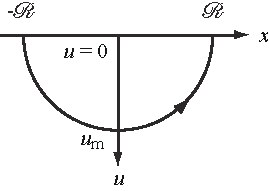
\includegraphics{Ch15_geodesic.pdf} }
\vskip2mm
\caption{The AdS$_3$ geodesic}
\label{fig:geodesic}
\end{figure}%
%%============

{\color{blue} 
\textit{Solution:}
The action becomes 
\be
%
\action = m \int du\, \frac{L}{u} \sqrt{x'^2+1}~.
%\label{eq:}
%
\ee
Then, the configuration is determined by
\be
%
x'^2 = \frac{y^2}{1-y^2}~, \qquad(y:=u/u_m)~,
%\label{eq:}
%
\ee
which can be easily integrated. One gets $u_m=\calR$, and the geodesic is a semi-circle $x^2+u^2=\calR^2$. 

Then, the action becomes
\begin{align}
%
\Sos &= 2mL \int_0^1 \frac{dy}{y\sqrt{1-y^2}} \\
&\simeq 2mL \ln \frac{2\calR}{\epsilon}.
%\label{eq:}
%
\end{align}
The result diverges, so we introduced the UV cutoff $u=\epsilon$.

This result has several applications. First, this gives an approximate two-point correlation function of an operator $\calO$ with $\Delta \gg 1$. From \eq{conf_weight_scalar}, $\Delta \gg 1$ implies $mL \gg 1$. Then, the scalar field is approximated by a massive point particle, and the two-point function becomes
\begin{align}
%
\bra \calO(\calR)\calO(-\calR) \ketc &\simeq e^{-\Sos} \\
&\simeq \frac{1}{R^{2mL}} \simeq \frac{1}{R^{2\Delta}}~,
%\label{eq:}
%
\end{align}
where the subscript ``$c$" represents the connected function. The result has the correct scaling dimension $2\Delta$.

Another application is the computation of the \keyword{holographic entanglement entropy} in AdS$_3$/CFT$_2$ \cite{Nishioka:2009un}.
}



%%%%%%%%%
\section*{Chap.~9}%\label{sec:}
%%%%%%%%%
%\setcounter{chapter}{3}
%\setcounter{prob}{0}

\begin{prob}
%\label{prob:}
\textbf{Density matrix and entropy} \\
From the density matrix $\rho$, the \keyword{von Newman entropy} is defined by
\be
%
S = -\text{tr} \left[ \rho \ln \rho \right]~.
%\label{eq:}
%
\ee
Using the canonical ensemble $\rho=e^{-\beta H}/Z$, show that $S$ indeed reduces to the thermodynamic entropy $S=\ln Z+ \beta H$.

For illustration, take the spin-1/2 systems in the text. For a pure ensemble, $S=0$. When $\rho$ is proportional to the identity operator $I$, the ensemble is called \keyword{maximally mixed}. The ensemble which contains  which contains $\kets{+}$ and $\kets{-}$ with equal weights is maximally mixed. In this case, $S=\ln2$. In general, $S \leq \ln d_{\calH}$, where $d_{\calH}$ is the dimensionality of the Hilbert space, and the equality is valid for a maximally mixed ensemble.
\end{prob}


\begin{prob}
\label{prob:bjorken}
\textbf{Bjorken flow (perfect fluid)} \\
We consider the time evolution of QGP using hydrodynamics. A heavy-ion collision is often approximated by a $(1\!+\!1)$-dimensional model $ds^2=-dT^2+dX^2$, where only the longitudinal beam direction $X$ is taken into account, and the transverse directions $(Y,Z)$ are ignored. The time evolution goes as follows (\fig{bjorken}):
\begin{itemize}
\item 
Because of ultra-relativistic nature, heavy-ions approximately move along light-cones $T=\pm X$.
\item
They collide at $(T,X)=(0,0)$ and pass through each other leaving behind excited quarks and gluons with various velocities. 
\item
The excited particles interact each other and reach a local equilibrium after some proper time $\tau_0$. (Time scales are determined by each particle's proper time $\tau$.) The particles then form QGP, and one is able to use hydrodynamics. 
\end{itemize}

%%============
\begin{figure}[tb]
\centering
%\hspace{0.25in}
\scalebox{0.55}{ 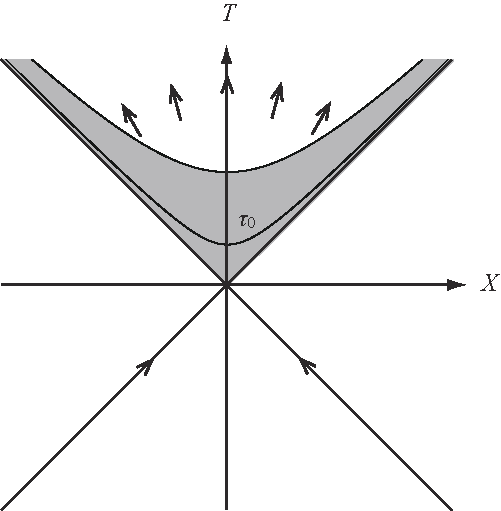
\includegraphics{Ch15_bjorken.pdf} }
\vskip2mm
\caption{The Bjorken flow. The shaded region represents excited particles and form QGP after $\tau_0$.}
\label{fig:bjorken}
\end{figure}%
%%============

A simple hydrodynamic model of the QGP evolution is known as the \keyword{Bjorken flow} \cite{Bjorken:1982qr}. In this model, each particle velocity is assumed to be $v=X/T$ or $u^\mu = (T,X)/\tau$. This configuration is boost-invariant, namely a different position of particles is simply Lorentz-boosted. It is also assumed that the fluid velocity $u^\mu(x)$ is given by the particle velocity there. In this exercise, we also assume a scale-invariant fluid where $T^\mu_{~\mu}=0$. We first consider the perfect fluid case. 

It is convenient to use the Milne coordinates \eqref{eq:milne} since it is the fluid rest frame. Adding transverse directions, 
\be
%
ds^2 = - d\tau^2 + \tau^2 dy^2 + dY^2 + dZ^2~.
\label{eq:milne2}
%
\ee

\noindent
(a) Show that a Lorentz boost acts as $y \rightarrow y+\text{constant}$, so the boost invariance means that physical quantities are $y$-independent. We will see that this is indeed the case. 

\noindent
(b) Write down $T^{\mu\nu}$ components in the Milne coordinates.

\noindent
(c) Derive hydrodynamic equations (continuity equation and Euler equation) for the Bjorken flow from the conservation equation $\nabla_\mu T^{\mu\nu}=0$. Note that the covariant derivative appears because the Milne coordinates do not take the Minkowski form. Solve hydrodynamic equations, and determine the time evolution of the energy density $\varepsilon$.

\noindent
(d) Determine the $\tau$-dependence of $s$ and $T$ using the Euler relation $\varepsilon+P=Ts$ and the first law $d\varepsilon = T ds$.
\end{prob}

{\color{blue} 
\textit{Solution:}
A Lorentz boost is given by $\tilde{x}^\mu = \Lambda^\mu_{~~\nu} x^\nu$, where
\be
%
\Lambda^\mu_{~~\nu} =
	\begin{pmatrix}
	  \cosh y & \sinh y  \\
	  \sinh y & \cosh y
	\end{pmatrix}
%\label{eq:}
%
\ee
(We consider only the $(T,X)$-directions.) Two successive boosts give 
\be
%
\Lambda^\mu_{~~\rho}(y) \Lambda^\rho_{~~\nu}(y') =
	\begin{pmatrix}
	  \cosh (y+y') & \sinh (y+y')  \\
	  \sinh (y+y') & \cosh (y+y')
	\end{pmatrix}~,
%\label{eq:}
%
\ee
so a boost acts as $y \rightarrow y+\text{constant}$.

The $T^{\mu\nu}$ components are given by
\begin{align}
%
 T^{\mu\nu} &= (\varepsilon+P)u^\mu u^\nu + P \eta^{\mu\nu} 
 \nonumber \\
 &\stackrel{RF}{=} 
	\begin{pmatrix}
	  \varepsilon & 0 & 0 & 0 \\
	  0 & \frac{P}{\tau^2} & 0 & 0 \\
	  0 & 0 & P & 0 \\
	  0 & 0 & 0 & P \\
	\end{pmatrix}~.
%\label{eq:}
%
\end{align}
The Euler equation reduces to
\be
%
\del_y P = 0~,
%\label{eq:}
%
\ee
so the pressure is $y$-independent or boost invariant. It then follows that the other thermodynamic quantities are all boost invariant. The continuity equation becomes
\be
%
\del_\tau \varepsilon + \frac{4}{3} \frac{\varepsilon}{\tau} = 0~,
%\label{eq:}
%
\ee
where $\epsilon=3P$ is used. Integrating the equation and using thermodynamic relations, one gets
\begin{align}
%
\varepsilon &\propto \tau^{-4/3}~,\\
s &\propto \tau^{-1}~,\\
T &\propto \tau^{-1/3}~.
%\label{eq:}
%
\end{align}
}


\begin{prob}
%\label{prob:}
\textbf{Bjorken flow (viscous fluid)} \\
Now, consider a viscous fluid case for the Bjorken flow. We again consider a scale-invariant fluid.

\noindent
(a) Write down $T^{\mu\nu}$ components in the Milne coordinates. One needs to evaluate $\nabla_\mu u_\nu$. 

\noindent
(b) Derive hydrodynamic equations from $\nabla_\mu T^{\mu\nu}=0$. 

\noindent
(c) Solving the continuity equation as a power series expansion in $1/\tau$, determine the large-$\tau$ behavior of $\varepsilon$.
\end{prob}

{\color{blue} 
\textit{Solution:}
The $T^{\mu\nu}$ components are given by
\be
%
T^{\mu\nu} 
\stackrel{RF}{=} 
	\begin{pmatrix}
	  \varepsilon & 0 & 0 & 0 \\
	  0 & \frac{P}{\tau^2} - \frac{4\eta}{3\tau^3} & 0 & 0 \\
	  0 & 0 & P + \frac{2\eta}{3\tau^3}  & 0 \\
	  0 & 0 & 0 & P + \frac{2\eta}{3\tau^3} \\
	\end{pmatrix}~.
%\label{eq:}
%
\ee
The $\nabla_\mu T^{\mu y}=0$ equation reduces to
\be
%
\del_y T^{yy} \propto \del_y P - \frac{4}{3\tau} \del_y \eta =0~,
%\label{eq:}
%
\ee
so a boost-invariant $P$ and $\eta$ satisfy the equation. The continuity equation becomes
\be
%
\del_\tau \varepsilon + \frac{4}{3} \frac{\varepsilon}{\tau} -  \frac{4}{3} \frac{\eta}{\tau^2} = 0~.
%\label{eq:}
%
\ee
The large-$\tau$ behavior is given by
\be
%
\varepsilon \propto \tau^{-4/3} - 2 \eta_0 \tau^{-2} + \cdots~,
%\label{eq:}
%
\ee
where $\eta_0$ is a constant which is related to $\eta$ as
\be
%
\eta = \frac{\eta_0}{\tau}~.
%\label{eq:}
%
\ee
$\eta$ depends on $\tau$ so is not a constant because $\eta$ is temperature-dependent:
\be
%
\eta \propto T^3 \propto \tau^{-1}~.
%\label{eq:}
%
\ee
}

%%%%%%%%%
\section*{Chap.~10}%\label{sec:}
%%%%%%%%%
%\setcounter{chapter}{3}
%\setcounter{prob}{0}

\begin{prob}
\label{prob:fieldop_Maxwell}
\textbf{Field/operator correspondence for the Maxwell field}\\
Consider the Maxwell field in the asymptotically AdS geometry:
\be
%
\action =  -\frac{1}{4} \int d^{p+2}x\, \sqrt{-g} F_{MN}^2~.
%
\ee
Following Sects.~\ref{sec:scalar} and \ref{sec:current}, derive the field/operator correspondence for the Maxwell field. Namely, evaluate the on-shell Maxwell action and compute $\cA$ in Eqs.~\eqref{eq:response_rho_ads} or \eqref{eq:response_current_ads}. The holographic renormalization is unnecessary for the Maxwell field.
\end{prob}

{\color{blue} 
\textit{Solution:}
\be
%
\bra J^x \ketj = (p-1) \vevA{x} \sourceA{x}~.
%\label{eq:}
%
\ee
or $\cA=p-1$. (We set $r_0=L=1$.) One can rewrite the result as
\be
%
A_x \sim \sourceA{x} + \frac{1}{p-1} \bra J^x \ketj\, u^{p-1}~,
\quad (u\rightarrow0)~.
%\label{eq:}
%
\ee
The scaling dimension of the current is $[J]=p$. The scaling dimension of the electric field $\sourceE = -\del_t \sourceA{x}$ is $[E]=2$. From the Ohm's law $J^x = \sigma \sourceE$, the scaling dimension of the conductivity is $[\sigma]=p-2$.
}

\begin{prob}
\label{prob:field_op_Lifshitz}
\textbf{Field/operator correspondence in the Lifshitz geometry}
\cite{Kachru:2008yh2,Taylor:2015glc} \\
The Lifshitz geometry is given by 
\begin{align}
%
ds^2 &= -r^{2z}dt^2 + r^2 d\bmx_p^2 + \frac{dr^2}{r^2} \\
&= - \frac{dt^2}{u^{2z}} + \frac{d\bmx_p^2}{u^2} + \frac{du^2}{u^2}~.
%\label{eq:}
%
\end{align}
The geometry is invariant under the anisotropic scaling
\be
%
t \rightarrow a^z t~, \bmx \rightarrow a \bmx~, u \rightarrow au~. \quad
(\text{or~}  r \rightarrow r/a)
%\label{eq:}
%
\ee

\noindent
(a) Consider the massless scalar field. Following \sect{scalar}, derive the field/operator correspondence: solve the equation of motion asymptotically, evaluate the on-shell action, and obtain the one-point function.

\noindent
(b) Consider the massive scalar field. Following \sect{massive_scalar}, solve the equation of motion asymptotically, and obtain the BF bound.

\noindent
(c) Derive the field/operator correspondence for the Maxwell field $A_x$.\\
\end{prob}

{\color{blue} 
\textit{Solution:}
For the massless scalar field,
\be
%
\phi \sim \source + \frac{1}{z+p} \bra \calO \ketj\, u^{z+p}~,
\quad (u\rightarrow0)~.
%\label{eq:}
%
\ee
The scaling dimension of $\bra \calO \ketj$ is $\Delta_+ = z+p$. This is because the perturbed action of the boundary theory $ \delta \action_\text{QFT} = \int d^{p+1}x\, \source \calO $ involves $d^{p+1}x$ which scales as $d^{p+1}x \rightarrow a^{z+p}d^{p+1}x$.

For the massive scalar field,
\begin{alignat}{2}
%
\phi &\sim\source u^{\Delta_-} + \cphi \bra\calO\ketj\, u^{\Delta_+}~,
&\quad& (u\rightarrow0)~,
 \\
\Delta_\pm &= \frac{z+p}{2} \pm \sqrt{\frac{(z+p)^2}{4}+m^2}~,&&
%
\end{alignat}
so the BF bound is given by
\be
%
m^2 \geq -\frac{(z+p)^2}{4}~.
%\label{eq:}
%
\ee

For the Maxwell field,
\be
%
A_x \sim \sourceA{x} + \frac{1}{z+p-2} \bra J^x \ketj\, u^{z+p-2}~,
\quad (u\rightarrow0)~.
%\label{eq:}
%
\ee
The scaling dimensions are $[J] = z+p-1$, $[E]=z+1$, and $[\sigma]=p-2$.
}


\begin{prob}
%\label{prob:}
\textbf{Temperature dependence of physical quantities in the Lifshitz geometry}\\
 We use the radial coordinate $r$ in this exercise. Consider the asymptotically Lifshitz black hole. Suppose that the horizon radius of the \bh satisfies the scaling $r_0 \rightarrow r_0/a$ like the SAdS black hole. Also, assume that $r_0$ or temperature $T$ is the only scale in the dual field theory. \\
 
\noindent
(a) Following \sect{SAdS}, obtain the temperature dependence of thermodynamic quantities.  Assume the area law, the first law, and the Euler relation. 
 
\noindent
(b) Similarly, using the result of \probset{field_op_Lifshitz}(c), obtain the temperature dependence of the conductivity $\sigma$.

\end{prob}

{\color{blue} 
\textit{Solution:}
\begin{align}
%
T &\simeq r_0^z~, \\
s &\simeq r_0^p \simeq T^{p/z}~, \\
\varepsilon &\simeq P \simeq T^{(z+p)/z}~, \\
\sigma &\simeq T^{(p-2)/z}~. 
%\label{eq:}
%
\end{align}
You do not need the explicit form of the \bh metric to know the dependence, but of course the biggest assumption is the scaling.

Including numerical coefficients, one can also show that $z\varepsilon=pP$ instead of $\varepsilon=pP$, which is a consequence of the anisotropic scaling.
}



%%%%%%%%%
\section*{Chap.~12}%\label{sec:}
%%%%%%%%%
%\setcounter{chapter}{3}
%\setcounter{prob}{0}

\begin{prob}
\label{prob:SAdS4_diff}
\textbf{Diffusion constant and conductivity for SAdS$_4$ black hole} \\
\prerequisite{\sect{SAdS5_diff} } \\
Consider the Maxwell field in the SAdS$_4$ background. Following \sect{SAdS5_diff}, obtain the conductivity $\sigma$ and the diffusion constant $D$ from the Maxwell vector mode computation. This exercise computes $\sigma$ for the holographic \SC\ in \chap{phase} in the high-temperature phase (in the probe limit).

\noindent
(a) Derive the $A_x$ equation from the Maxwell equation. Solve the equation of motion up to $O(\omega)$. Expand the solution asymptotically keeping the terms of $O(u)$.  One may use \textit{Mathematica} for this problem.

\noindent 
(b) Obtain $\sigma$ from \eq{fast_vs_cond_ads5}. Also, obtain $\chi_T$ and $D$. \\

\end{prob}


{\color{blue} 
\textit{Solution:} 
The $A_x$ equation is written as
\be
%
\frac{1}{h}(h A_x')' + \frac{\omega^2}{\Ts^2 h^2} A_x = 0~,
%\label{eq:}
%
\ee
where $h=1-u^3$ and $\Ts:=4\pi T/3=r_0/L^2$. This is \eq{Ax_eom_4} with $\Psi=0$. The solution asymptotically behaves as 
\be
%
A_x = \sourceA{x} \left\{ 1 + \frac{i\omega}{\Ts} u + \cdots \right\}~, 
\qquad (u\rightarrow 0)~.
%\label{eq:}
%
\ee

$\vevA{x} = i \omega/\Ts$, so 
\be
%
\sigma = \frac{\cA}{\Ts} = 1~.
\label{eq:cond_ads4} 
%
\ee
The factor $\cA$ has been computed in \probset{fieldop_Maxwell}. Recovering dimensionful quantities, $\cA=\Ts$. [We set the normalization factor $\alpha=1$ in \eq{action_Maxwell}.] Finally,
\begin{align}
%
\chi_T &= \cA = \Ts~, \\
D &= \frac{\sigma}{\chi_T} = \frac{1}{\Ts} = \frac{3}{4\pi T}~.
%\label{eq:}
%
\end{align}
}


\begin{prob}
\label{prob:2nd}
\textbf{Second-order transport coefficients for the \Nfour\ SYM} 
\cite{Baier:2007ix3} \\
\prerequisite{Sects.~\ref{sec:Lorentzian_prescription} and \ref{sec:action_tensor} } \\
One can derive second-order transport coefficients \eqref{eq:transport_causal} from the tensor mode response $\delta \bra \tau^{xy}  \ket $.

\noindent
(a) Following \sect{action_tensor}, compute the on-shell tensor mode action up to $O(\omega^2,q^2)$. You need to reevaluate the counterterm action. \\

{\color{blue} 
\textit{Solution:} 
We set $r_0=L=16\pi G_5=1$ in this problem. 
\be
%
\Sos = \left. V_4 + \left(-\frac{1}{2} + \frac{q^2-\omega^2}{4u^2} \right) \phim\cdot\phip+\frac{1}{2u^3}\phim\cdot\phip'  \right|_{u=0}~
%\label{eq:}
%
\ee
instead of \eq{tensor_on_shell1}.\\
}

\noindent
(b) Following \sect{tensor_mode_sol}, solve the tensor mode equation of motion up to $O(\omega^2,q^2)$. Expand the solution asymptotically keeping the terms of $O(u^4)$. One may use \textit{Mathematica} for this problem.\\

{\color{blue} 
\textit{Solution:}
Write the solution as $\phi_k = \source_k f_k(u)$. Then, 
\be
%
f_k = 1 - \frac{q^2-\omega^2}{4} u^2 + \frac{1}{4} \left\{i\omega + \frac{1}{2}q^2 - \frac{1-\ln 2}{2} \omega^2 \right\} u^4 + \cdots~, \qquad (u\rightarrow 0)~.
%f_k = 1 + \frac{1}{4} i\omega u^4 + \frac{1}{8} q^2 u^2 (-2+u^2) + \frac{1}{8} \omega^2 u^2 \{ 2-u^2(1-\ln 2) \} + \cdots~, \qquad (u\rightarrow 0)~.
%\label{eq:}
%
\ee
}

\noindent
(c) Following \sect{Lorentzian_prescription}, substitute the solution into the on-shell action and obtain 
$\delta \bra \tau^{xy}  \ket $. Comparing with the Kubo formula \eqref{eq:kubo_causal}, obtain $\kappa$ and $\tau_\pi$. \\

{\color{blue} 
\textit{Solution:} 
In the convention of \sect{Lorentzian_prescription}, the fluctuation-dependent on-shell action becomes
\begin{align}
%
%\Sos[\source] = \int (dk) \left.\phim^{(0)}\, \Fp\, \phip^{(0)} \right|_{u=0}^{u=1}~, \quad
\Sos[\source] &= \int (dk)\, \phim^{(0)} \left\{
\left. \Fp \right|_{u=0} - \left.\Fp \right|_{u=1} 
\right\} \phip^{(0)}~,
%\label{eq:bdy_bc} 
\\
\left. 2\Fp \right|_{u=0} &= \left. \left( -1 + \frac{q^2-\omega^2}{2u^2} \right) f_{-k}f_{k} 
+ \frac{1}{u^3} f_{-k}f_{k}' \right|_{u=0}
\\
& = -1 + i\omega + \frac{1}{2}q^2 - \frac{1-\ln 2}{2} \omega^2 + \cdots~.
\label{eq:def_Fk2}
%\label{eq:}
%
\end{align}
Recall that the response is written as
\be
%
\bra \calO_k  \ketj = \left. 2\Fp \right|_{u=0} \source_k~.
\tag{\ref{eq:Lorentzian_prescription}}
%\label{eq:Lorentzian_prescription2}
%
\ee
Comparing with the Kubo formula, one gets
$P=\eta=\kappa=1$, and
$\tau_\pi =(2-\ln2)/2$.
}
\end{prob}

\textit{Further suggestions:} Similarly, compute transport coefficients for SAdS$_4$ and SAdS$_7$ black holes \cite{Natsuume:2008iy}:
\begin{alignat}{3}
%
P&=\eta=1, \tau_\pi =  1-\frac{\ln 3 -\frac{\sqrt{3} \pi}{9}}{2} &
\qquad &(\text{SAdS$_4$}) \\
P&=\eta=1, \tau_\pi = 1-\frac{\ln 3 +\frac{\sqrt{3} \pi}{9}}{4}~,~ &\kappa =\frac{1}{2}
\qquad &(\text{SAdS$_7$}) 
%\label{eq:}
%
\end{alignat}
The result of $\tau_\pi$ can be summarized using the harmonic number $H_n = \sum_{k=1}^n \frac{1}{k}$ as follows \cite{Natsuume:2008gy}:
\be
%
\tau_\pi = \frac{1}{2} + \frac{H_{\frac{2}{p+1}}}{p+1}~.
%\label{eq:}
%
\ee



%%%%%%%%%
\section*{Chap.~13}%\label{sec:}
%%%%%%%%%
%\setcounter{chapter}{3}
%\setcounter{prob}{0}

\begin{prob}
\label{prob:factorization}
\textbf{Large-$\Nc$ factorization}\\
Consider a two-point correlation function of an operator%
\footnote{More precisely, we consider the so-called single-trace operators such as $\calO \simeq \text{tr} F^2$. In this book, we consider only single-trace operators.} 
$\calO$
\be
%
\bra \calO\calO \ket = \bra\calO\ket \bra\calO\ket + \bra \calO\calO \ketc~,
%\label{eq:}
%
\ee
where the subscript ``$c$" represents the connected correlation function. Argue that the first term is $O(\Nc^4)$ whereas the second term is $O(\Nc^2)$ using AdS/CFT. 

This property is known as \keyword{large-$\Nc$ factorization}. Although large-$\Nc$ gauge theories are strongly-coupled, gauge invariant operators are weakly-coupled, and their interactions are suppressed by $1/\Nc$. They are classical and behaves as $c$-numbers in the large-$\Nc$ limit.
\end{prob}

\newcommand{\Sosd}{\underline{I}}

{\color{blue} 
\textit{Solution:}
This behavior essentially comes from the fact that the Newton's constant appears only as the overall coefficient of the bulk action. Let us introduce the dimensionless metric $ds^2 =L^2 ds^2_\text{dimensionless}$. Then, the bulk action becomes
\begin{align}
%
\action &= \frac{1}{16\pi G_5} \int d^5x \sqrt{-g} R + \cdots 
\\
&= \frac{L^3}{16\pi G_5} S_\text{dimensionless}
\simeq \Nc^2 S_\text{dimensionless}~.
%\label{eq:}
%
\end{align}
The action is proportional to $\Nc^2$
%: this overall coefficient affects the field/operator correspondence. 
which implies
\begin{align}
%
\bra \calO \ketnoj &
= \left.\frac{\delta Z}{\delta \source}\right|_{\source=0} 
%= \Nc^2 \left.\frac{\delta \Sosd}{\delta \source}\right|_{\source=0}
\simeq \Nc^2~.\\
\bra \calO\calO \ketc &
= -\left.\frac{\delta^2 W}{\delta \phi^{(0)2}}\right|_{\source=0} 
%= -\Nc^2 \left.\frac{\delta^2 \Sosd}{\delta \phi^{(0)2}}\right|_{\source=0}
\simeq \Nc^2~,
%\label{eq:}
%
\end{align}
where $Z = \bra e^{-\source\calO} \ket$, $W$ is the generating function of connected correlation functions given by $Z=e^{-W}$ (it is essentially the bulk on-shell action), and we use the Euclidean formalism.
Thus,
\begin{alignat}{2}
%
\bra\calO\calO\ket  
 = &\bra \calO \ket \bra \calO \ket 
 + &\bra \calO\calO \ketc~. \\
 &\quad\Nc^4 & \Nc^2 \qquad\nonumber
%
\end{alignat}


The argument here is formal in character. But, for example, we computed the one-point function of the energy-momentum tensor:
\be
%
\bra T_{\mu\nu}\ket 
 \simeq \Nc^2~.
%\label{eq:}
%
\ee
We also computed the one-point function in the presence of the source which is related to the two-point function via the linear response theory:
\be
%
\delta \bra T_{xy}\ket
 \simeq \bra T_{xy}T_{xy}\ketc
 \simeq \Nc^2~.
%\label{eq:}
%
\ee
%Thus,
%\begin{alignat}{2}
%
%\bra T_{\mu\nu}T_{\rho\sigma}\ket  
% = &\bra T_{\mu\nu}\ket \bra T_{\rho\sigma}\ket 
% + &\bra T_{\mu\nu} T_{\rho\sigma}\ketc~. \\
% &\qquad\Nc^4 & \Nc^2 \qquad\nonumber
%
%\end{alignat}
(Here, we were sloppy about the differences among various correlators/Green's functions. We have mostly computed retarded Green's functions, but all others can be obtained once the retarded Green's function is known.)
}

\begin{prob}
\label{prob:ginzburg}
\textbf{Ginzburg criterion}\\
The large-$\Nc$ factorization does not hold for field theory in general, but a similar property holds when the number of spatial dimensions are large enough. The mean-field theory utilizes this property. Again, compare connected and disconnected correlation functions. We would like to know when the following condition is satisfied:
%The mean-field theory ignores the fluctuations of the order parameter. Let us estimate the validity of the assumption. The fluctuations are suppressed when
\be
%
\bra m(\bmx) \ket \bra m(\bm{0}) \ket \gg \bra m(\bmx) m(\bm{0}) \ketc~.
%\label{eq:}
%
\ee
Show that the condition leads to the Ginzburg criterion:
\be
%
m^2 \xi^{\ds} \gg T\chi_T~,
%\label{eq:}
%
\ee
In terms of critical exponents, one gets \eq{critical_dim}:
\be
%
\ds \geq d_\text{UC} = \frac{2\beta+\gamma}{\nu}~.
%\label{eq:}
%
\ee
%In large-$\Nc$ gauge theories, the Ginzburg criterion is satisfied because of the large-$\Nc$ factorization (\probset{factorization}).
\end{prob}

{\color{blue} 
\textit{Solution:}
Integrating the equation over the region with size $\xi$, one gets
\begin{align}
%
\int_0^\xi d\bmx\, \bra m(\bmx) \ket \bra m(\bm{0}) \ket
 &\simeq m^2 \xi^{\ds}~,
\\
\int_0^\xi d\bmx\, \bra m(\bmx) m(\bm{0}) \ketc
 &\simeq \int_0^\infty d\bmx\, T \chi(\bmx) = T\chi_T~.
%\label{eq:}
%
\end{align}
}


%%%%%%%%%
\section*{Chap.~14}%\label{sec:}
%%%%%%%%%
%\setcounter{chapter}{3}
%\setcounter{prob}{0}

\begin{prob}
%\label{prob1}
\textbf{Hawking-Page transition of SAdS$_4$ black hole}\\
The SAdS$_4$ black hole with $S^2$ horizon is given by
\be
%
ds_4^2 =  - \left( \frac{r^2}{L^2} + 1 - \frac{r_0^3}{L^2r} \right) dt^2 
+ \frac{dr^2}{ \frac{r^2}{L^2} + 1 - \frac{r_0^4}{L^2r} } 
+ r^2 d\Omega_2^2~.
%\label{eq:}
%
\ee
Compute the free energy using two methods below and discuss the Hawking-Page transition.

\noindent
(a) Following \sect{HP_S3}, compute free energy using the reference spacetime method.

\noindent
(b) (\prerequisite{\sect{SAdS_free}}) Following \sect{SAdS_free}, compute free energy. Is there a Casimir energy in this case?
\end{prob}

{\color{blue} 
\textit{Solution:}
\be
%
F =  - \frac{\ro}{4G_4 L^2} (\ro^2-L^2)~.
%\label{eq:}
%
\ee
}

\begin{prob}
%\label{prob1}
\textbf{Free energy of Schwarzschild black hole} \\
\prerequisite{\sect{SAdS_free} } \\
Compute the free energy of the four-dimensional Schwarzschild black hole and verify \eq{free_Sch}. 

First, following \sect{SAdS_free}, compute the Gibbons-Hawking action. (The on-shell bulk action vanishes.) In order to obtain a finite free energy, use the reference spacetime method in \sect{HP_S3} instead of the counterterm method. Use the flat spacetime for the reference spacetime.
\end{prob}

\begin{prob}
%\label{prob1}
\textbf{Critical temperature in alternative quantization} \\
\prerequisite{Sects.~\ref{sec:massive_more} and \ref{sec:HSC_more} } \\
In the text, we consider the asymptotic behavior
\be
%
\psi_1 \sim \psi_1^{(0)} u + \cpsi \bra\calO_2\ketj\, u^2~,
\quad (u\rightarrow0)~.
%\label{eq:}
%
\ee
This is the so-called standard quantization. But when
\be
%
- \frac{9}{4} \leq m^2 \leq - \frac{5}{4} \quad(\text{for~} p=2)~,
%\label{eq:}
%
\ee
(For the holographic \SC, $m^2=-2$, so this condition is satisfied), the slow falloff is also normalizable so that one can exchange the role of the external source and the operator. Namely, one can consider
\be
%
\psi_1 \sim \cpsi \bra\calO_1\ketj\, u + \psi_1^{(0)} u^2~,
\quad (u\rightarrow0)~.
%\label{eq:}
%
\ee
This is the so-called alternative quantization. The scaling dimensions are $[\calO_2]=2$ and $[\calO_1]=1$. 

Following \sect{HSC_more}, compute the critical temperature in the alternative quantization by imposing $\psi_1^{(0)}=0$. One may use \textit{Mathematica}.
\end{prob}

{\color{blue} 
\textit{Solution:}
\begin{align}
%
\frac{\Ts_c}{\mu} &\approx 0.893~, \quad(\text{for } \calO_1)~, \\ %0.8925
\textit{cf. } \frac{\Ts_c}{\mu} &\approx 0.246~, \quad(\text{for } \calO_2)~. %0.24608
%\label{eq:}
%
\end{align}
In general, the critical temperature rises as the scaling dimension of the order parameter becomes smaller.
}

\begin{thebibliography}{99}

%
% Chap_exercises 
%

% again
%\cite{Rey:1998bq}
\bibitem{Rey:1998bq2}
  S.~-J.~Rey, S.~Theisen and J.~-T.~Yee,
  ``Wilson-Polyakov loop at finite temperature in large N gauge theory and anti-de Sitter supergravity,''
  Nucl.\ Phys.\ B {\bf 527} (1998) 171
  [hep-th/9803135].
  %%CITATION = HEP-TH/9803135;%%

% again
%\cite{Brandhuber:1998bs}
\bibitem{Brandhuber:1998bs2}
  A.~Brandhuber, N.~Itzhaki, J.~Sonnenschein and S.~Yankielowicz,
  ``Wilson loops in the large N limit at finite temperature,''
  Phys.\ Lett.\ B {\bf 434} (1998) 36
  [hep-th/9803137].
  %%CITATION = HEP-TH/9803137;%%
  
% again
%\cite{Herzog:2006gh}
\bibitem{Herzog:2006gh2}
  C.~P.~Herzog, A.~Karch, P.~Kovtun, C.~Kozcaz and L.~G.~Yaffe,
  ``Energy loss of a heavy quark moving through N=4 supersymmetric Yang-Mills plasma,''
  JHEP {\bf 0607} (2006) 013
  [hep-th/0605158].
  %%CITATION = HEP-TH/0605158;%%

%\cite{Herzog:2006se}
\bibitem{Herzog:2006se}
  C.~P.~Herzog,
  ``Energy Loss of Heavy Quarks from Asymptotically AdS Geometries,''
  JHEP {\bf 0609} (2006) 032
  [hep-th/0605191].
  %%CITATION = doi:10.1088/1126-6708/2006/09/032;%%  

%\cite{Nishioka:2009un}
\bibitem{Nishioka:2009un}
  T.~Nishioka, S.~Ryu and T.~Takayanagi,
  ``Holographic Entanglement Entropy: An Overview,''
  J.\ Phys.\ A {\bf 42} (2009) 504008
  [arXiv:0905.0932 [hep-th]].
  %%CITATION = doi:10.1088/1751-8113/42/50/504008;%%

%\cite{Bjorken:1982qr}
\bibitem{Bjorken:1982qr}
  J.~D.~Bjorken,
  ``Highly Relativistic Nucleus-Nucleus Collisions: The Central Rapidity Region,''
  Phys.\ Rev.\ D {\bf 27} (1983) 140.
%  doi:10.1103/PhysRevD.27.140
  %%CITATION = doi:10.1103/PhysRevD.27.140;%%
  
% again
%\cite{Kachru:2008yh}
\bibitem{Kachru:2008yh2}
  S.~Kachru, X.~Liu and M.~Mulligan,
  ``Gravity Duals of Lifshitz-like Fixed Points,''
  Phys.\ Rev.\ D {\bf 78} (2008) 106005
  [arXiv:0808.1725 [hep-th]].
  %%CITATION = ARXIV:0808.1725;%%

%\cite{Taylor:2015glc}
\bibitem{Taylor:2015glc}
  M.~Taylor,
  ``Lifshitz holography,''
  Class.\ Quant.\ Grav.\  {\bf 33} (2016) no.3,  033001
  [arXiv:1512.03554 [hep-th]].
  %%CITATION = doi:10.1088/0264-9381/33/3/033001;%%
  
% again2
%\cite{Baier:2007ix}
\bibitem{Baier:2007ix3}
  R.~Baier, P.~Romatschke, D.~T.~Son, A.~O.~Starinets and M.~A.~Stephanov,
  ``Relativistic viscous hydrodynamics, conformal invariance, and holography,''
  JHEP {\bf 0804} (2008) 100
  [arXiv:0712.2451 [hep-th]].
  %%CITATION = JHEPA,0804,100;%%

%\cite{Natsuume:2008iy}
\bibitem{Natsuume:2008iy}
  M.~Natsuume and T.~Okamura,
  ``A Note on causal hydrodynamics for M-theory branes,''
  Prog.\ Theor.\ Phys.\  {\bf 120} (2008) 1217
  [arXiv:0801.1797 [hep-th]].
  %%CITATION = doi:10.1143/PTP.120.1217;%%

%\cite{Natsuume:2008gy}
\bibitem{Natsuume:2008gy}
  M.~Natsuume,
  ``Causal hydrodynamics and the membrane paradigm,''
  Phys.\ Rev.\ D {\bf 78} (2008) 066010
  [arXiv:0807.1392 [hep-th]].
  %%CITATION = doi:10.1103/PhysRevD.78.066010;%%
  
\end{thebibliography}

\endofsection

\begin{prob}
%\label{prob1}
\textbf{}\\
\end{prob}

{\color{blue} 
\textit{Solution:}
}
